\chapter{Выбор компонентов}

По результатам расчетов были выбраны:
\begin{enumerate}
\item	операционный усилитель \textbf{OPA27}
\item	резисторы \textbf{ CF-100} (С1-4) номиналом 10 кОм.
\end{enumerate}

\begin{figure}[h!]
	\centering
	\caption{Параметры операционного усилителя }
	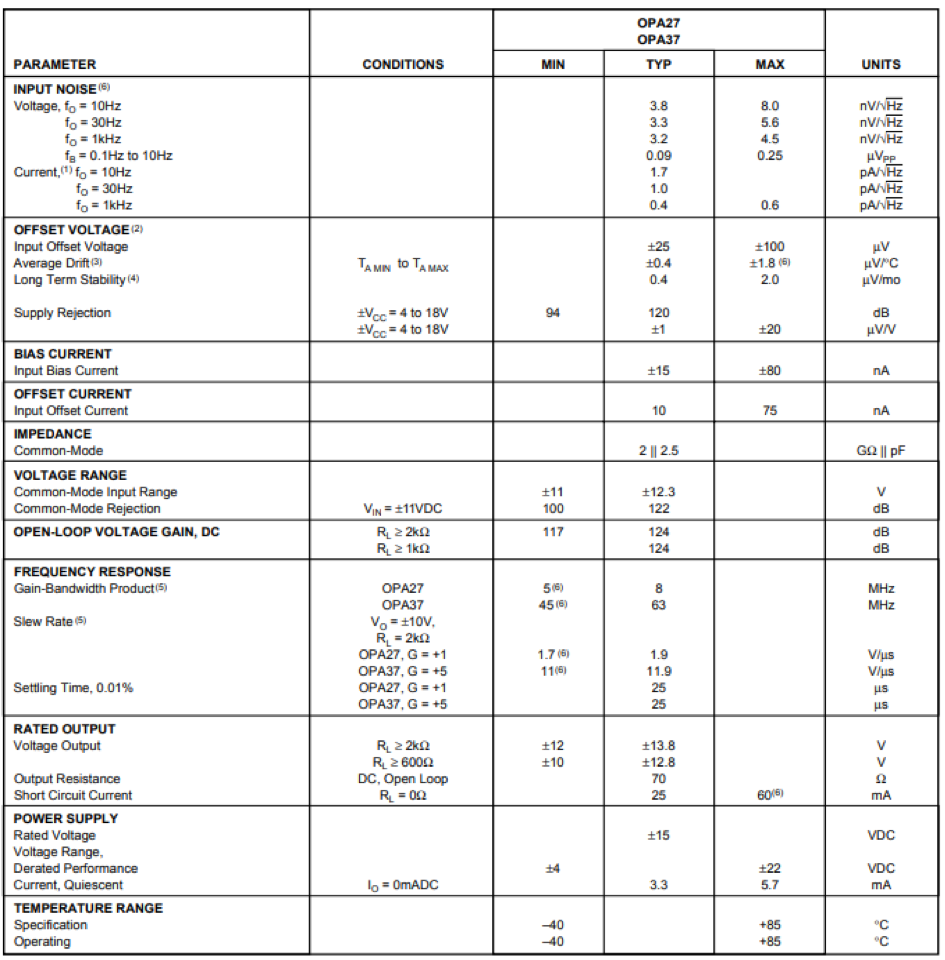
\includegraphics{images/1.png}
\end{figure}

\begin{figure}[h!]
	\centering
	\label{fig2}
	\caption{Зависимость коэффициента усиления от частоты}
	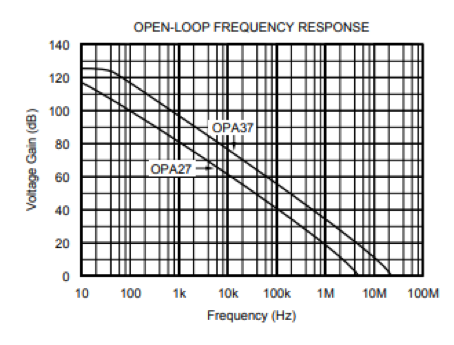
\includegraphics{images/2.png}
\end{figure}

\begin{figure}[h!]
	\centering
	\caption{Параметры резистора CF-100 (С1-4)}
	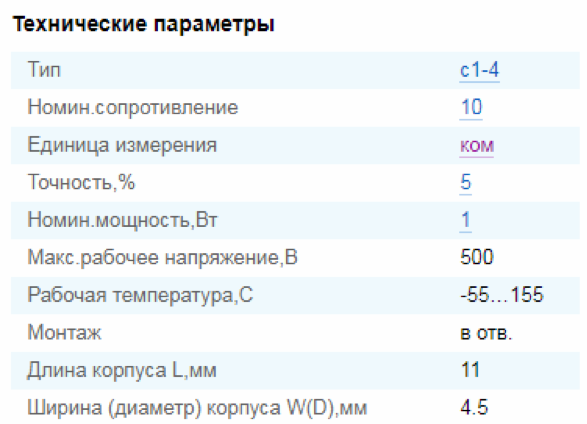
\includegraphics{images/3.png}
\end{figure}
